\begin{figure}[htbp]
  \centering
  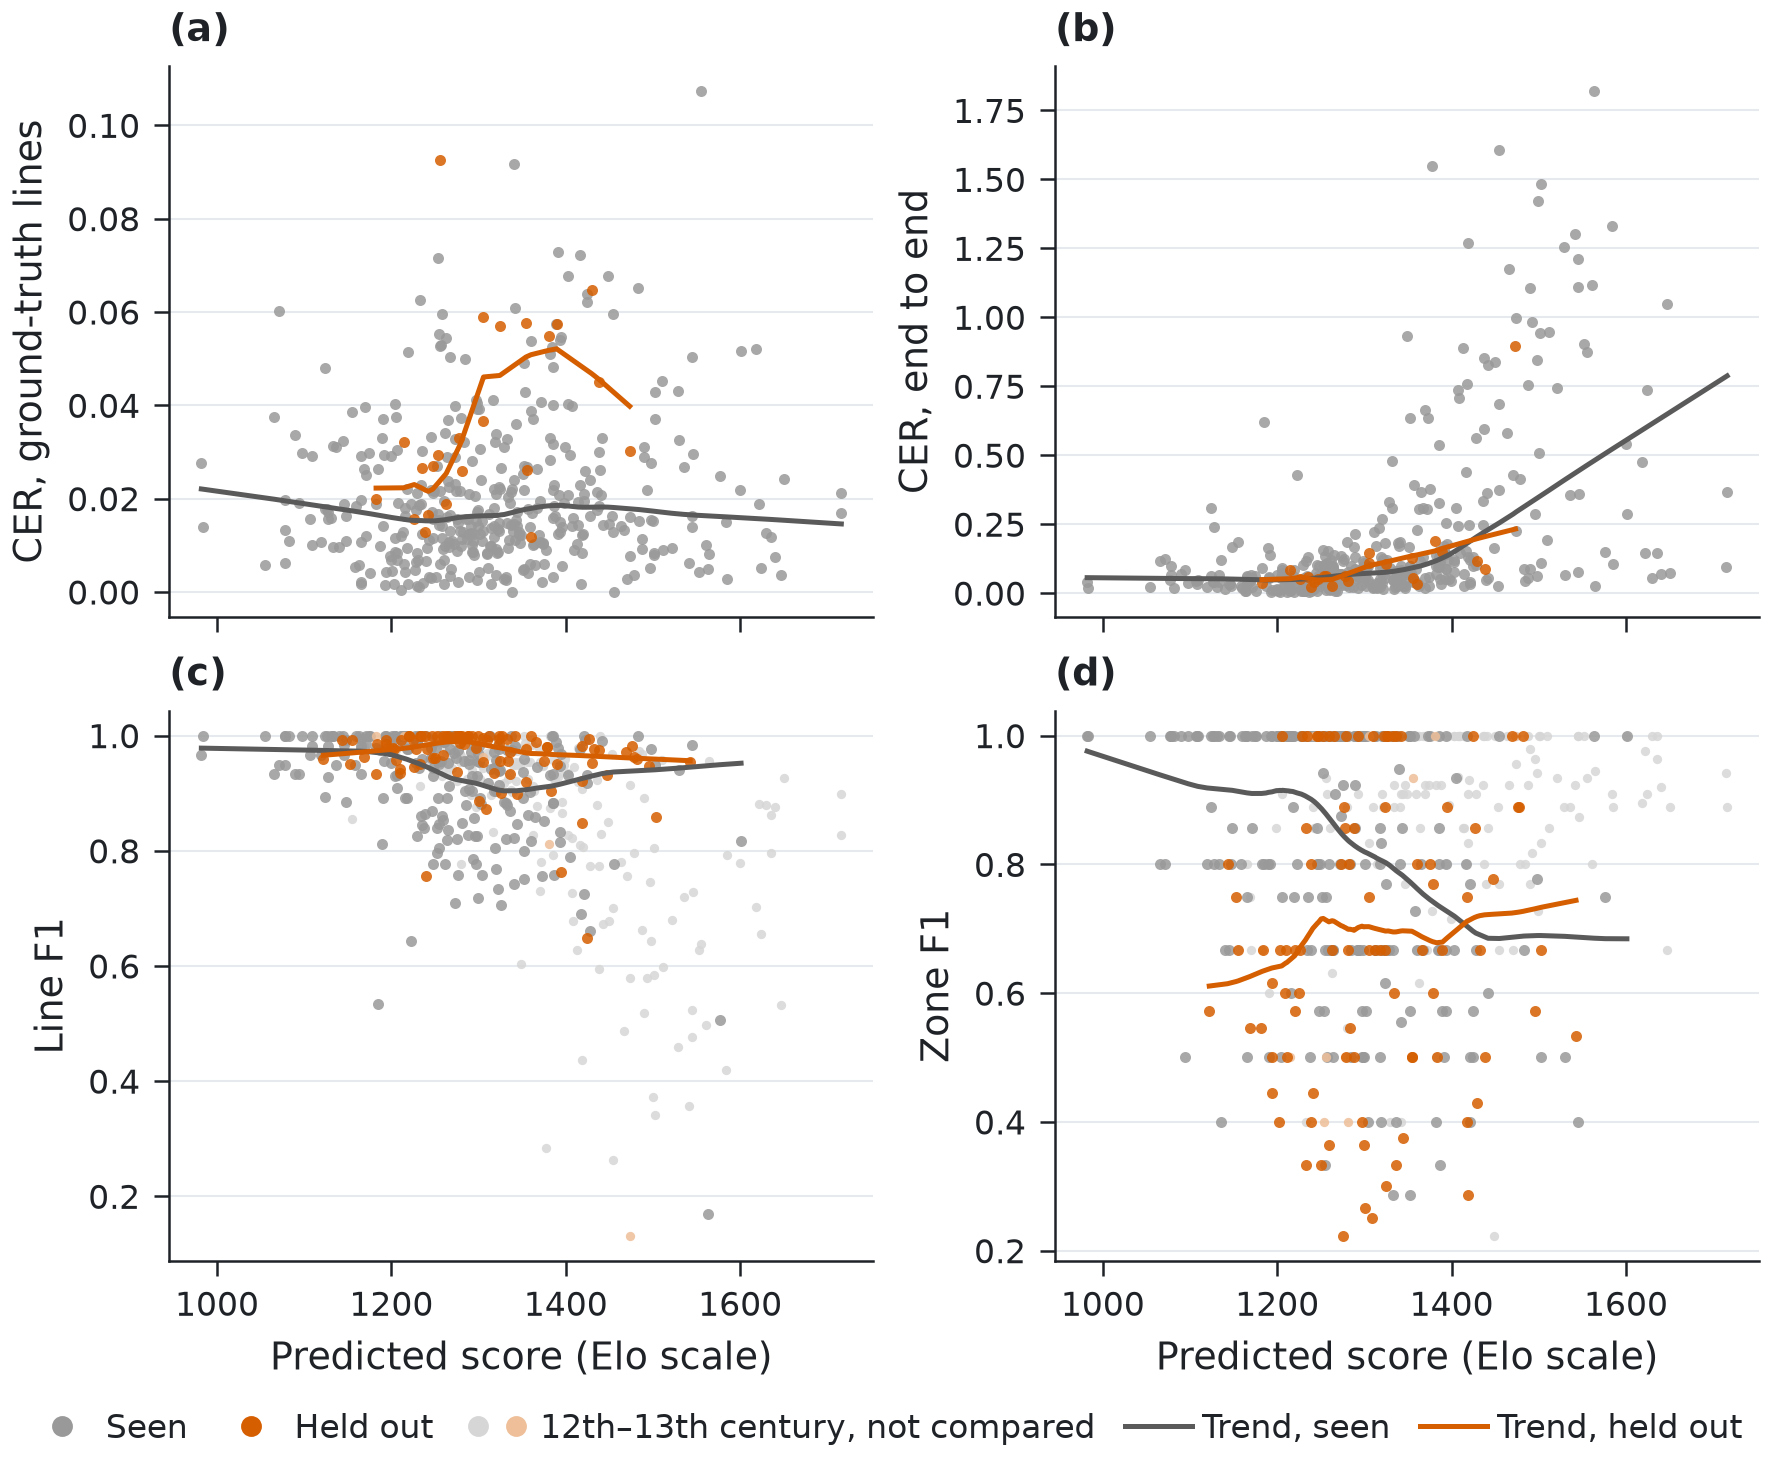
\includegraphics[width=15.00cm]{figures/difficulty_against_complexity.png}
  \caption{Automatic difficulty against predicted complexity, each dot a page: (a) the character error rate (CER) of Kraken with CATMuS Medieval's model on the ground-truth lines and (b) end to end, on Kraken's own lines; (c) line F1 of Kraken's lines and (d) zone F1 of the regions model's zones, against the ground truth. (a) and (b) show CREMMA's 412 pages with a CER, (c) and (d) CREMMA's 418 and the 83 pages of CATMuS's test split from its handwritten manuscripts of the 14th to 16th century. Left out: 1 page whose ground truth has no text line (every line a drop capital's or music's). The CERs leave out 5 pages whose ground-truth texts don't fit their lines: at least 3 text lines read, on Kraken's line matched to them, as the text of the line just before or after (a CER over 50\% against their own text, under 25\% against the neighbour's), or read as empty through their own polygon while Kraken's line reads text. Grey: pages CATMuS's models trained on; vermillion: held out, in CATMuS's test split (23 of CREMMA's, from 4 manuscripts). The lines are robust LOWESS trends of each group, each local fit over 50\% of the group's pages with three robustifying iterations; in (c) and (d) over the pages of the 14th to 16th century, both sides, CREMMA's 12th- and 13th-century pages lighter and outside them. Predicted complexity is the expected Elo score of the shipped ensemble: a prediction, for nobody judged these pages. The regions model and the recognition model trained on 395 of CREMMA's 418 pages. Zone F1 is the F1 score of the regions model's zones against the ground truth's, matched one to one within each class by the IoU of boxes (from 0.5); line F1 that of Kraken's lines against the ground truth's text lines (default, heading and interlinear), matched by the IoU of polygons, a found line matching a drop capital's or music's counting neither way; the baseline distance, the mean distance between matched baselines in line heights; the CER, the character error rate of Kraken with CATMuS Medieval's model, on the ground-truth lines and end to end (on Kraken's lines, missed lines' characters and invented lines' added), texts in NFC with whitespace runs as one space.}
  \label{fig:difficulty_against_complexity}
\end{figure}
